\begin{figure}[tbp]
        \centering
        \resizebox{0.4\linewidth}{!}{%
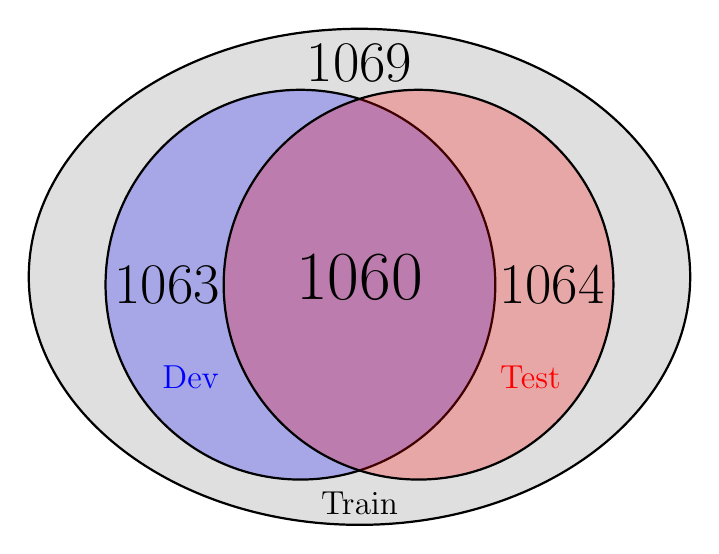
\begin{tikzpicture}[ 
    set/.style = {draw, circle,
        minimum size = 4.95cm}]
\draw (0.75cm,0.1cm) ellipse (4.2cm and 3.15cm) [
    set,
    fill = gray,
    fill opacity = 0.25,
    text opacity = 1,
    %label={[label distance=0.01cm]90:\large Train},
    thick
    ] node (TRAIN) {};
\node (DEV) [
    set,
    fill = blue,
    fill opacity = 0.25,
    text opacity = 1,
    label = {[label distance=-1.2cm,blue]225:\large Dev},
    thick
    ] {};
% \node (B) at (45:3.25cm) [
%     set,
%     minimum size = 11.5cm,
%     fill = gray,
%     fill opacity = 0.25,
%     text opacity = 1,
%     label={[label distance=0.01cm]90:\large Train},
%     thick
%     ] {\Huge \bf $1069$};
\node (TEST) at (0:1.5cm) [
    set,    
    fill = red,
    fill opacity = 0.25,
    text opacity = 1,
    label={[label distance=-1.2cm,red]315:\large Test},
    thick
    ] {};
 
\node at (DEV.center) [left,xshift=-0.9cm] {\huge $1063$};
\node at (TRAIN.center) {\Huge $1060$};
\node at (TRAIN.center) [below, yshift=-2.6cm]{\large Train};
\node at (TRAIN.center) [above, yshift=2.35cm]{\huge $1069$};
\node at (TEST.center) [right,xshift=0.9cm] {\huge $1064$};
% \node at (B.north) [above, yshift=-3.5cm] {\Large $1069$};
% \node at (barycentric cs:A=1,B=0.1,C=1) [] {3};
\end{tikzpicture}%
}
        \caption{\small Number of videos per train, dev, and test corpus of Signing in the Wild, splitting as proposed by~\cite{borg_sign_2019}. Numbers in the overlapping regions indicate video/signer overlaps between the sets. \vspace{-4mm}}
        \label{fig:datasets_signinginthewildoriginal_overlap}
    \end{figure}